\documentclass{article}

\usepackage[dutch]{babel}
\usepackage[margin=3cm]{geometry}
\usepackage{graphicx}
\usepackage{float}
\usepackage{caption}
\usepackage{hyperref}
\usepackage{amsmath}
\usepackage{wrapfig}
\usepackage[parfill]{parskip}
\usepackage{eso-pic}

% fonts
\usepackage[T1]{fontenc}
\usepackage{helvet}
\renewcommand{\familydefault}{\sfdefault}

\graphicspath{{img/}}


% code
\usepackage{minted}
\setminted{frame=single,framesep=3pt,linenos}
\usepackage{upquote}
\usepackage{color}

\definecolor{titlepagecolor}{RGB}{68,200,245}

\begin{document}

\begin{titlepage}
    \pagecolor{titlepagecolor}
    \newgeometry{left=3cm,right=1cm,bottom=1cm}
    \noindent
\begin{flushright}
\vspace*{5cm}
 \vspace{2cm}
\end{flushright}
    \color{white}
    \par
    \noindent
    \color{white}
    \makebox[0pt][l]{\rule{1.3\textwidth}{1pt}}
    \par\medskip
    {\noindent \Huge\textbf{\textsf{Installation guide: Research project}}}
    \par\medskip
    {\noindent\Large\textsf{Pieter Specenier}}
    \par  
\vfill%


\end{titlepage}
\restoregeometry

\nopagecolor 

\pagenumbering{gobble}
\tableofcontents
\newpage

\pagenumbering{arabic}

% Add watermark to background of every page
\AddToShipoutPicture{
    \ifnum\value{page}>0
    \AtPageLowerLeft{
    \raisebox{3\baselineskip}{\makebox[0.25\paperwidth]{
        \begin{minipage}{21cm}\centering
            
\includegraphics{img/background.png}
        \end{minipage}}}
    }
  \fi
}

\section{Installation}
The installation of the software is done by the following steps:
\begin{enumerate}
\item Clone the github repository on to your computer through this link on my \href{https://github.com/PieterSpecenier/Researchproject2022}{github}.
\item Now navigate to the cloned repository and run the following command: pip install -r requirements.txt
\item After installing all the requirements you can now run the app.py file, located in the API folder. 
\begin{figure}[H]
    \centering
    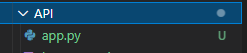
\includegraphics[width=0.6\textwidth]{apiapp.png}
    \caption{API app file location}
\end{figure}
\item After making sure the app is up and running you can now access the API through the following link: C:/Users/{USERNAME}/Documents/GitHub/Researchproject2022/researchproject/frontend/index.html
\item You can also find this link by clicking on the copy path button and pasting it into your browser.
\begin{figure}[H]
    \centering
    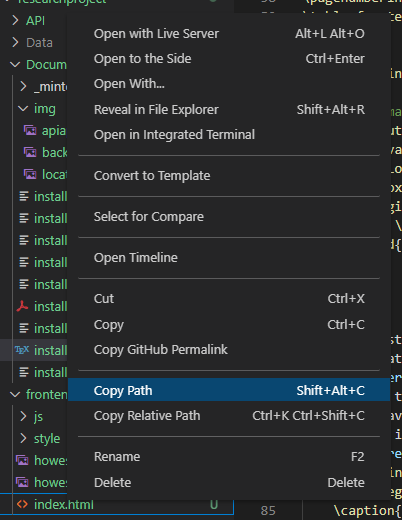
\includegraphics[width=0.4\textwidth]{locationwebsite.PNG}
    \caption{How to get to website of API}
\end{figure}
\item If every worked according to plan you should now have the following website in front of you
\begin{figure}[H]
    \centering
    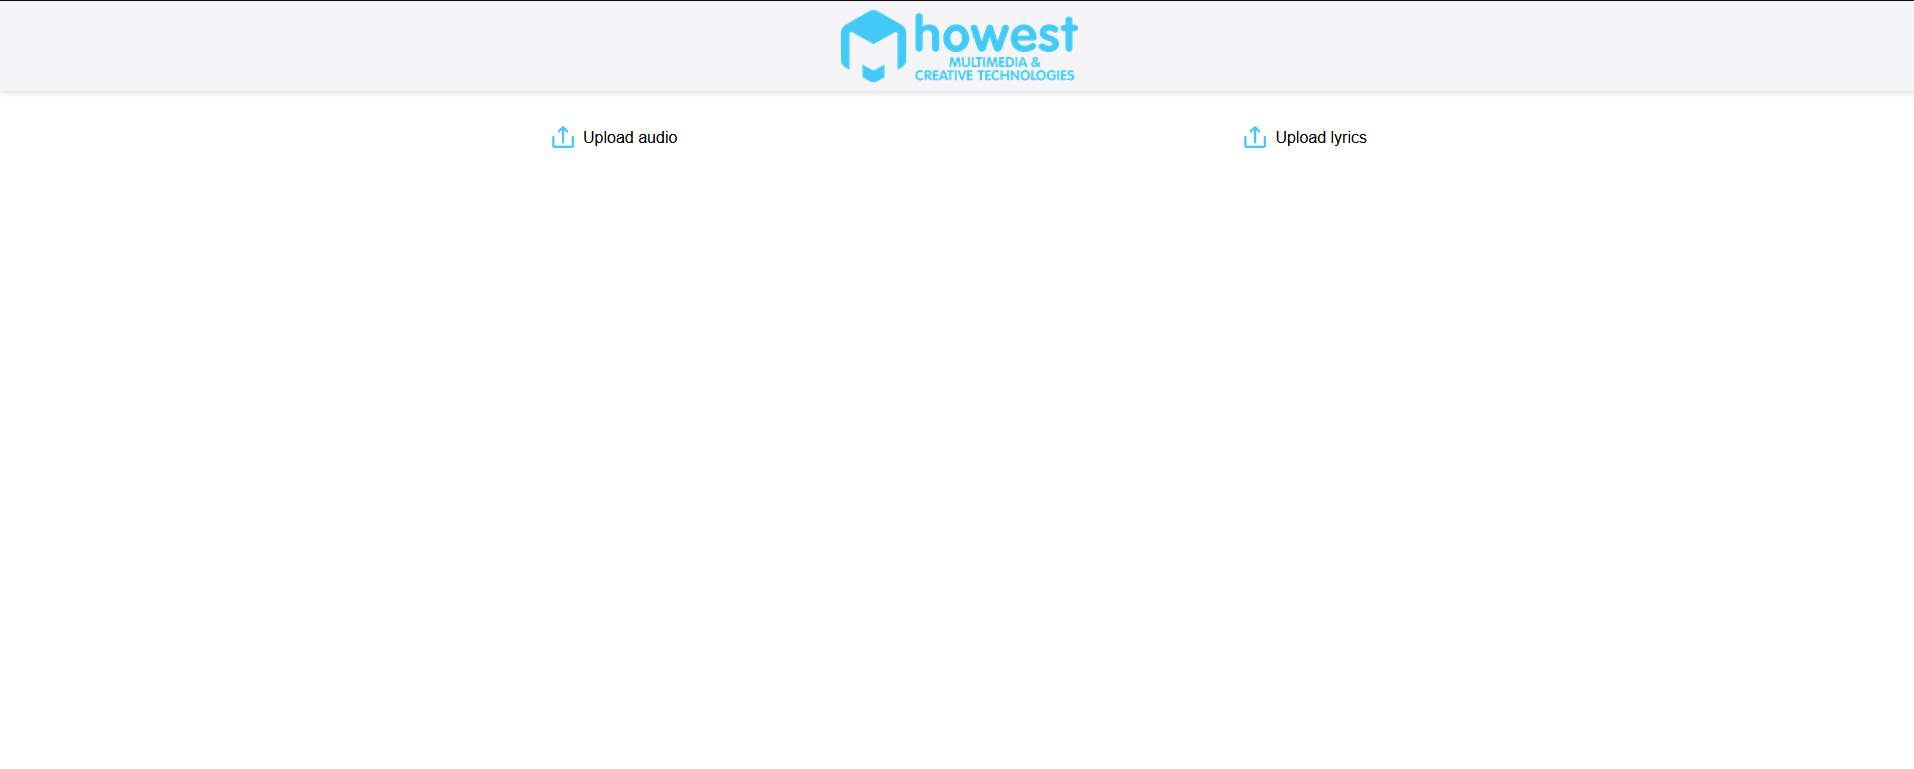
\includegraphics[width=0.6\textwidth]{website.PNG}
    \caption{View of the website}
\end{figure}
\item Have fun with the API!
\end{enumerate}

\end{document}